\documentclass[12pt]{article}
\usepackage{inputenc}
\usepackage[top=1in, bottom=1in, left=1in, right=1in]{geometry}
\usepackage{setspace}
\usepackage{parskip}
\setcounter{secnumdepth}{1}
\pagestyle{plain}
\usepackage{graphicx}
%\usepackage{fontspec}
%\setmainfont{Georgia}
\setlength{\parindent}{0 cm}
\usepackage[section]{placeins}


\usepackage[compact]{titlesec}  
\usepackage{amssymb}
\usepackage{amsmath}
\newcommand\numberthis{\addtocounter{equation}{1}\tag{\theequation}}
\titlespacing{\section}{0pt}{0pt}{0pt}
\usepackage{changepage}
\newenvironment{myenv}{\begin{adjustwidth}{1cm}{}}{\end{adjustwidth}}

\begin{document}
% Manual Heading
{\raggedleft{}Gabriel Griggs} \\
Professor Mark Alber \\
Nonlinear Dynamical Systems: ACMS 403630 --- 01 \\
Thursday, January 30th 2014\\
Homework 1
\section*{Question 1}
\begin{myenv}
\textbf{Question:} Consider a differential equation $ \dot{x} = f(x) = ax - x^3$ for some $a \in \mathbb{R}$. Determine fixed points and their stability for cases where $a$ is positive, negative, and zero.

\textbf{Answer:} In order to determine the fixed points, we must set $ f(\bar{x}) = 0 $ and solve for $ \bar{x} $. This yields:
\begin{align*}
f(\bar{x}) = 0 = a\bar{x}-\bar{x}^3 = x(a-\bar{x}^2)
\end{align*}
\begin{align*}
\bar{x} = 0, \pm\sqrt{a}
\end{align*}

Thus, our fixed points are going to be located at $\bar{x} = 0$ and $\pm\sqrt{a}$. In order to determine the stability at each of these points for the three cases of a, we will graph them using $a = 4, a = 0$ and $a = -4$ as representative cases.

Our first case $ a = 4 $, represents the case where $ a > 0 $. Seen in the graphs below, this scenario yields stable fixed points at $ \pm\sqrt(a) $ and an unstable node at $a = 0$. For $a = 0$, we have one stable node at the origin. Finally, for the $ a < 0 $ case, we use $ a = -4 $ as a proxy. This graph reveals a similar one to the $ a = 0 $ case in that there is a stable node at the origin.

\begin{figure} [H]
    \centering
    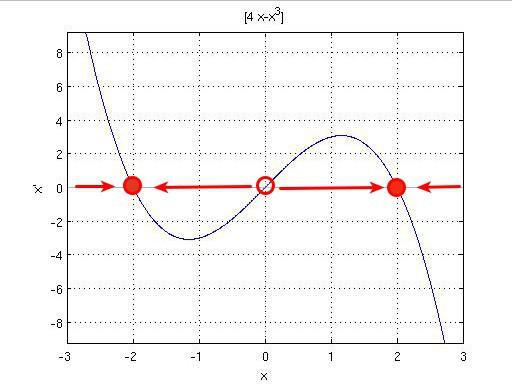
\includegraphics[width=0.8\textwidth]{a41}
    \caption{$ a > 0$ represented by $ a = 4 $}
    \label{figure:a1}
\end{figure}

\begin{figure} [H]
    \centering
    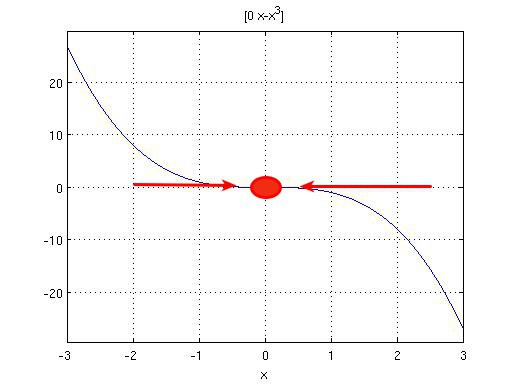
\includegraphics[width=0.8\textwidth]{a0}
    \caption{ $ a = 0$}
    \label{figure:a0}
\end{figure}

\begin{figure} [H]
    \centering
    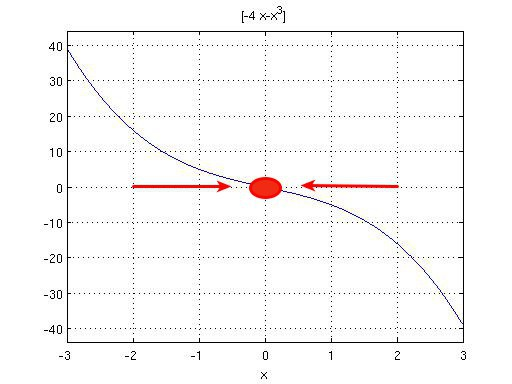
\includegraphics[width=0.8\textwidth]{anegative4}
    \caption{ $ a = 0$}
    \label{figure:a0}
\end{figure}

\end{myenv}

\section*{Question 2}
\begin{myenv}
\textbf{Question:} Find fixed points and sketch nullclines, vector field and plausible phase portrait of the system:
\begin{alignat*}{3}
\dot{x} &= x(x-y) &= f(x,y) \\
\dot{y} &= y(2x-y) &= g(x,y)
\end{alignat*}


\textbf{Answer:} In order to find the fixed points, we need to find $(\bar{x},\bar{y})$ such that $f(\bar{x},\bar{y}) = 0$ and $g(\bar{x},\bar{y}) = 0$. Thus, the only fixed point occurs at $(0,0)$.

The Jacobian matrix at a general point in this system is given as:
\begin{align*}
	J &= 
	\begin{Bmatrix}
	2x-y & -x \\
	2y & -2y + 2x
	\end{Bmatrix}
\end{align*}

Evaluating the Jacobian at the fixed point $(0,0)$ yields:
\begin{align*}
	J &= 
	\begin{Bmatrix}
	0 & 0 \\
	0 & 0
	\end{Bmatrix}, 	&\Lambda^2 &= 0,	&\Lambda &= 0, &det &= 0, &trace &= 0
\end{align*}


This analysis tells us that linearization of our system predicts a center at $(0,0)$. However, by looking at a graph of the vector field and the null clines (at lines $x = 0, y = 0,$ and $y = 2x$), reveals that there is not a center (or at least, not a typical center). This graph can be seen below. 

The fact that this is not a typical center becomes even clearer when we look at the vector field graph with possible solutions overlaid. It appears that initial conditions in the 1st and 3rd quadrants return to the origin, while initial solutions in the 2nd and 4th quadrant go to infinity. This graph can be seen, with the caption ``Phase Portrait'', below.

Note: In the final graph below, the vector field that is predicted by linearization has been extrapolated far past the origin, so we should not expect the actual system to follow these predictions (and they do not).



\begin{figure} [H]
    \centering
    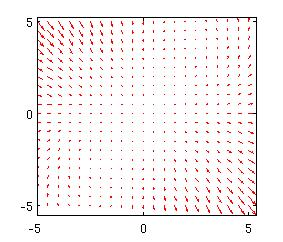
\includegraphics[width=0.8\textwidth]{Question2_VectorField}
    \caption{ Vector Field and Nullclines}
    \label{figure:a0}
\end{figure}


\begin{figure} [H]
    \centering
    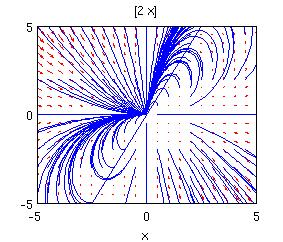
\includegraphics[width=0.8\textwidth]{Question2_PhasePortrait}
    \caption{ Phase Portrait}
    \label{figure:a0}
\end{figure}
\end{myenv}

\section*{Question 3}
\textbf{Question:} Show that the following system is reversible:
\begin{alignat*}{3}
\dot{x} &= y(1-x^2) &= f(x,y)\\
\dot{y} &= 1-y^2 &= g(x,y)
\end{alignat*}
\textbf{Answer:} We can show that this system is reversible by showing that $f(x,-y) = -f(x,y)$ and $g(x,-y) = g(x,y)$, as seen below.

\begin{alignat*}{3}
f(x,-y) &= -y(1-x^2) = -f(x,y) \\
g(x,-y) &= 1 - (-y)^2 = 1-y^2 = g(x,y)
\end{alignat*}

\section*{Question 4}
\begin{myenv}
\textbf{Question:} Is the origin a nonlinear center of the system?
\begin{alignat*}{3}
\dot{x} &= -y-x^2 &= f(x,y)\\
\dot{y} &= x &= g(x,y)
\end{alignat*}
\textbf{Answer:} Yes, the origin is a nonlinear center to this system. This center can be found by linearization of this system and can be verified by looking at a vector field / phase portrait.

The linearization process consists in verifying that $(0,0)$ is a fixed point and then evaluating the Jacobian of this system at the $(0,0)$ and calculating the resulting eigenvalues.

The Jacobian matrix at a general point in this system is given as:
\begin{align*}
	J &= 
	\begin{Bmatrix}
	-2x & -1 \\
	1 & 0
	\end{Bmatrix}
\end{align*}

Evaluating the Jacobian at the fixed point $(0,0)$ yields:
\begin{align*}
	J &= 
	\begin{Bmatrix}
	0 & -1 \\
	1 & 0
	\end{Bmatrix}, 	&\Lambda^2 &= -1,	&\Lambda &= \pm i, &det &= 1, &trace &= 0
\end{align*}

Since the $det>0$ and the $trace=0$, by linearization the fixed point $(0,0)$ would be classified as a center. In order to verify this, we overlay the phase portrait on the vector field. With initial conditions starting at $(.1,.1)$ the system returns a closed orbit around the fixed point, which is expected behavior for a fixed point. This closed orbit verifies that the fixed point at $(0,0)$ is indeed a center.

This system can explicitly be shown to have a \emph{nonlinear center} by showing that this system is reversible under the transformations $x \mapsto -x$ and $y \mapsto -y$.

\begin{alignat*}{3}
f(-x,y) &= -y-(-x)^2 = -y-(x)^2 = f(x,y) \\
g(-x,y) &= (-x) = -g(x,y)
\end{alignat*}

And (the back of the book agrees that this system is reversible. I cannot figure out how $f(x,-y) = -f(x,y)$, however.)
\begin{alignat*}{3}
f(x,-y) &= - (-y) - x^2 =? -f(x,y) = -(-y-x^2) = y+x^2 \\
g(x,-y) &= x = g(x,y)
\end{alignat*}

If this system is indeed reversible, then we can use Thm 6.61 (Strogatz) to prove that this is a robust \emph{nonlinear center}.


\begin{figure} [H]
    \centering
    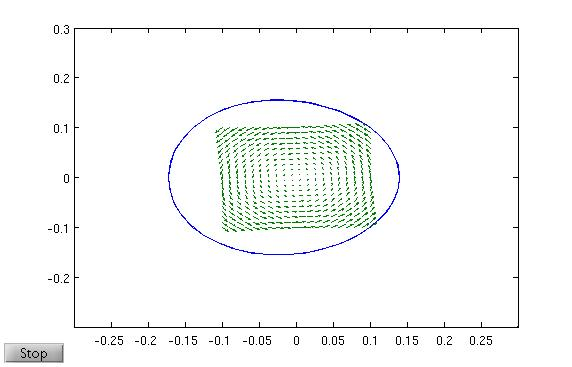
\includegraphics[width=0.8\textwidth]{Question4_Center}
    \caption{ Phase Portrait}
    \label{figure:a0}
\end{figure}
\end{myenv}

\section*{Question 5}
\begin{myenv}
\textbf{Question:} Study the Lotka-Voltera predator-prey model given by the system of equations:
\begin{alignat*}{3}
\dot{R} &= aR - bRF \\
\dot{F} &= -cF + dRF
\end{alignat*}
a) Show that the model can be recast in a non-dimensional form:
\begin{alignat*}{3}
\dot{x} &= x(1-y) \\
\dot{y} &= \mu y(x-1)
\end{alignat*}
b) Plot the vector field of the system.
c) Discuss the biological relevance of solutions of the system.
\textbf{Answer:} 
a) 


\end{myenv}
\end{document}

